\section{Le CERN}\label{chapter-LHC-section-CERN}
\subsection{Les origines du CERN}
L'acronyme \og CERN \fg{} signifie Conseil Européen pour la Recherche Nucléaire.
Sa création est motivée par l'état de la recherche scientifique en Europe après la Seconde Guerre Mondiale~\cite{CERN_website}.
Des scientifiques comme Raoul Dautry, Pierre Auger ou Niels Bohr envisagent la création d'un laboratoire européen de physique atomique\footnote{À cette époque, la physique fondamentale est la physique atomique et nucléaire, la physique des particules telle qu'elle est connue aujourd'hui n'est pas encore née.} n'ayant aucune motivation militaire.
Leur objectif est de stopper la fuite des cerveaux vers l'Amérique, d'unifier l'Europe et lui donner les moyens d'avoir une infrastructure de recherche en physique de calibre mondial.
\par Le 9 décembre 1949, Louis de Broglie propose officiellement la création d'un laboratoire européen.
C'est en décembre 1951, lors d'une conférence de l'UNESCO à Paris, qu'est adoptée une résolution pour la mise en place d'un conseil européen pour la recherche nucléaire avec pour objectif de créer une convention pour un laboratoire européen sous 18 mois.
Le site de Meyrin, au Nord-Ouest de Genève, est choisi en octobre 1952 pour sa position centrale vis-à-vis des pays européens et la neutralité militaire suisse. Les travaux commencent dès le printemps 1954.
\par Lors de la sixième session du Conseil Européen pour la Recherche Nucléaire, la convention établissant l'organisation européenne pour la recherche nucléaire est adoptée par les douze pays membres fondateurs: la Belgique, le Danemark, la France, la Grèce, l'Italie, la Norvège, les Pays-Bas, la République Fédérale d'Allemagne, le Royaume-Uni, la Suède, la Suisse et la Yougoslavie.
La ratification est terminée le 29 septembre 1954.
Le Conseil Européen pour la Recherche Nucléaire est alors dissous, mais l'acronyme CERN est resté attaché à l'organisation européenne pour la recherche nucléaire.
\subsection{Réalisations du CERN}
Le CERN a permis de réaliser de nombreuses découvertes en physique fondamentale, comme
les courants neutres~\cite{Hasert:243640,HASERT1973138,Hasert:203096} (1973),
les bosons \Wboson\ et \Zboson (1983, Nobel 1984) \cite{Wboson_discovery1,Wboson_discovery2,Wboson_discovery3,Zboson_discovery1,Zboson_discovery2}
et dernièrement le boson de Higgs (2012, Nobel 2013) \cite{ATLAS_Higgs_discovery,CMS_Higgs_discovery}.
\par En plus de découvertes majeures en physique fondamentale, le CERN apporte également des innovations technologiques importantes.
Par exemple, les techniques de hadronthérapie pour le traitement des tumeurs cancéreuses sont en grande partie développées au CERN.
Plus connus du grand public, les écrans tactiles ont été développés dans les années 70 au CERN afin de réduire le nombre de boutons dans la salle de contrôle du Supersynchrotron à Protons~\cite{CERN_touchscreen}.
Le Web a également été développé au CERN~\cite{CERN_web}.
\subsection{Les accélérateurs du CERN}
Le premier accélérateur de particules du CERN est le Synchrocyclotron, mis en service en 1957 à une énergie de \SI{600}{\MeV}.
Il est remplacé en 1990 par ISOLDE.
\par À la fin des années 50, le Synchrotron à Protons (PS) permet d'accélérer des protons et d'atteindre une énergie de \SI{28}{\GeV}, ce qui en fait l'accélérateur le plus puissant à l'époque.
Avec l'arrivée de nouveaux anneaux au CERN, le PS sert également de pré-accélérateur.
\par En 1976, le Supersynchrotron à Protons (SPS) est mis en service.
Le tunnel circulaire de \SI{7}{\kilo\meter} de circonférence permet de faire collisionner deux faisceaux de particules circulant en sens inverse avec une énergie dans le centre de masse allant jusqu'à \SI{450}{\GeV} pour des protons.
Le SPS a permis entre autres d'étudier la structure interne du proton et de découvrir les bosons
\Wboson~\cite{Wboson_discovery1,Wboson_discovery2,Wboson_discovery3}
et
\Zboson~\cite{Zboson_discovery1,Zboson_discovery2}.
\par Une nouvelle étape est franchie à la fin des années 80 avec la mise en service du Grand Collisionneur Électron-Positron (LEP, \emph{Large Electron-Positron collider}).
Il est, à ce jour, le plus grand collisionneur de leptons au monde avec \SI{27}{\kilo\meter} de circonférence.
Quatre grandes expériences étaient installées sur le LEP,
ALEPH~\cite{aleph_paper} (\emph{Apparatus for LEP PHysics at CERN}), 
DELPHI~\cite{delphi_paper} (\emph{DEtector with Lepton, Photon and Hadron Identification})
L3~\cite{l3_paper} et
OPAL~\cite{opal_paper} (\emph{Omni-Purpose Apparatus at LEP}),
dont les emplacements sont visibles sur la figure~\ref{fig-CERN_map} avec ceux des grandes expériences du LHC.
Le LEP a permis de réaliser des mesures de précision sur les bosons \Wboson\ et \Zboson\ précédemment découverts avec le SPS.
Il a été mis en arrêt en 2000 afin de construire le LHC, sujet de la section suivante.
\par De nombreuses autres expériences et installations expérimentales sont présentes au CERN dont le complexe d'accélérateurs s'étend sur près de \SI{10}{\kilo\meter}.
Sur la figure~\ref{fig-chapter-LHC-section-CERN-CERN_Accelerator-Complex} se trouve une carte de ce complexe avec les différentes structures encore en fonctionnement à ce jour.
\begin{figure}[p]
\centering
\includegraphics[width=.8\textwidth]{\PhDthesisdir/plots_and_images/CERN_and_LHC/CERN_LHC_LEP_and_experiments_map-scale_2km.tex}
\caption[Emplacements des grandes expériences du LEP et du LHC.]{Emplacements des grandes expériences du LEP (1989-2000) et du LHC (depuis 2008)~\cite{CERN_map}. Les tracés des \emph{booster}, PS et SPS sont également visibles.}
\label{fig-CERN_map}

\vspace{2\baselineskip}

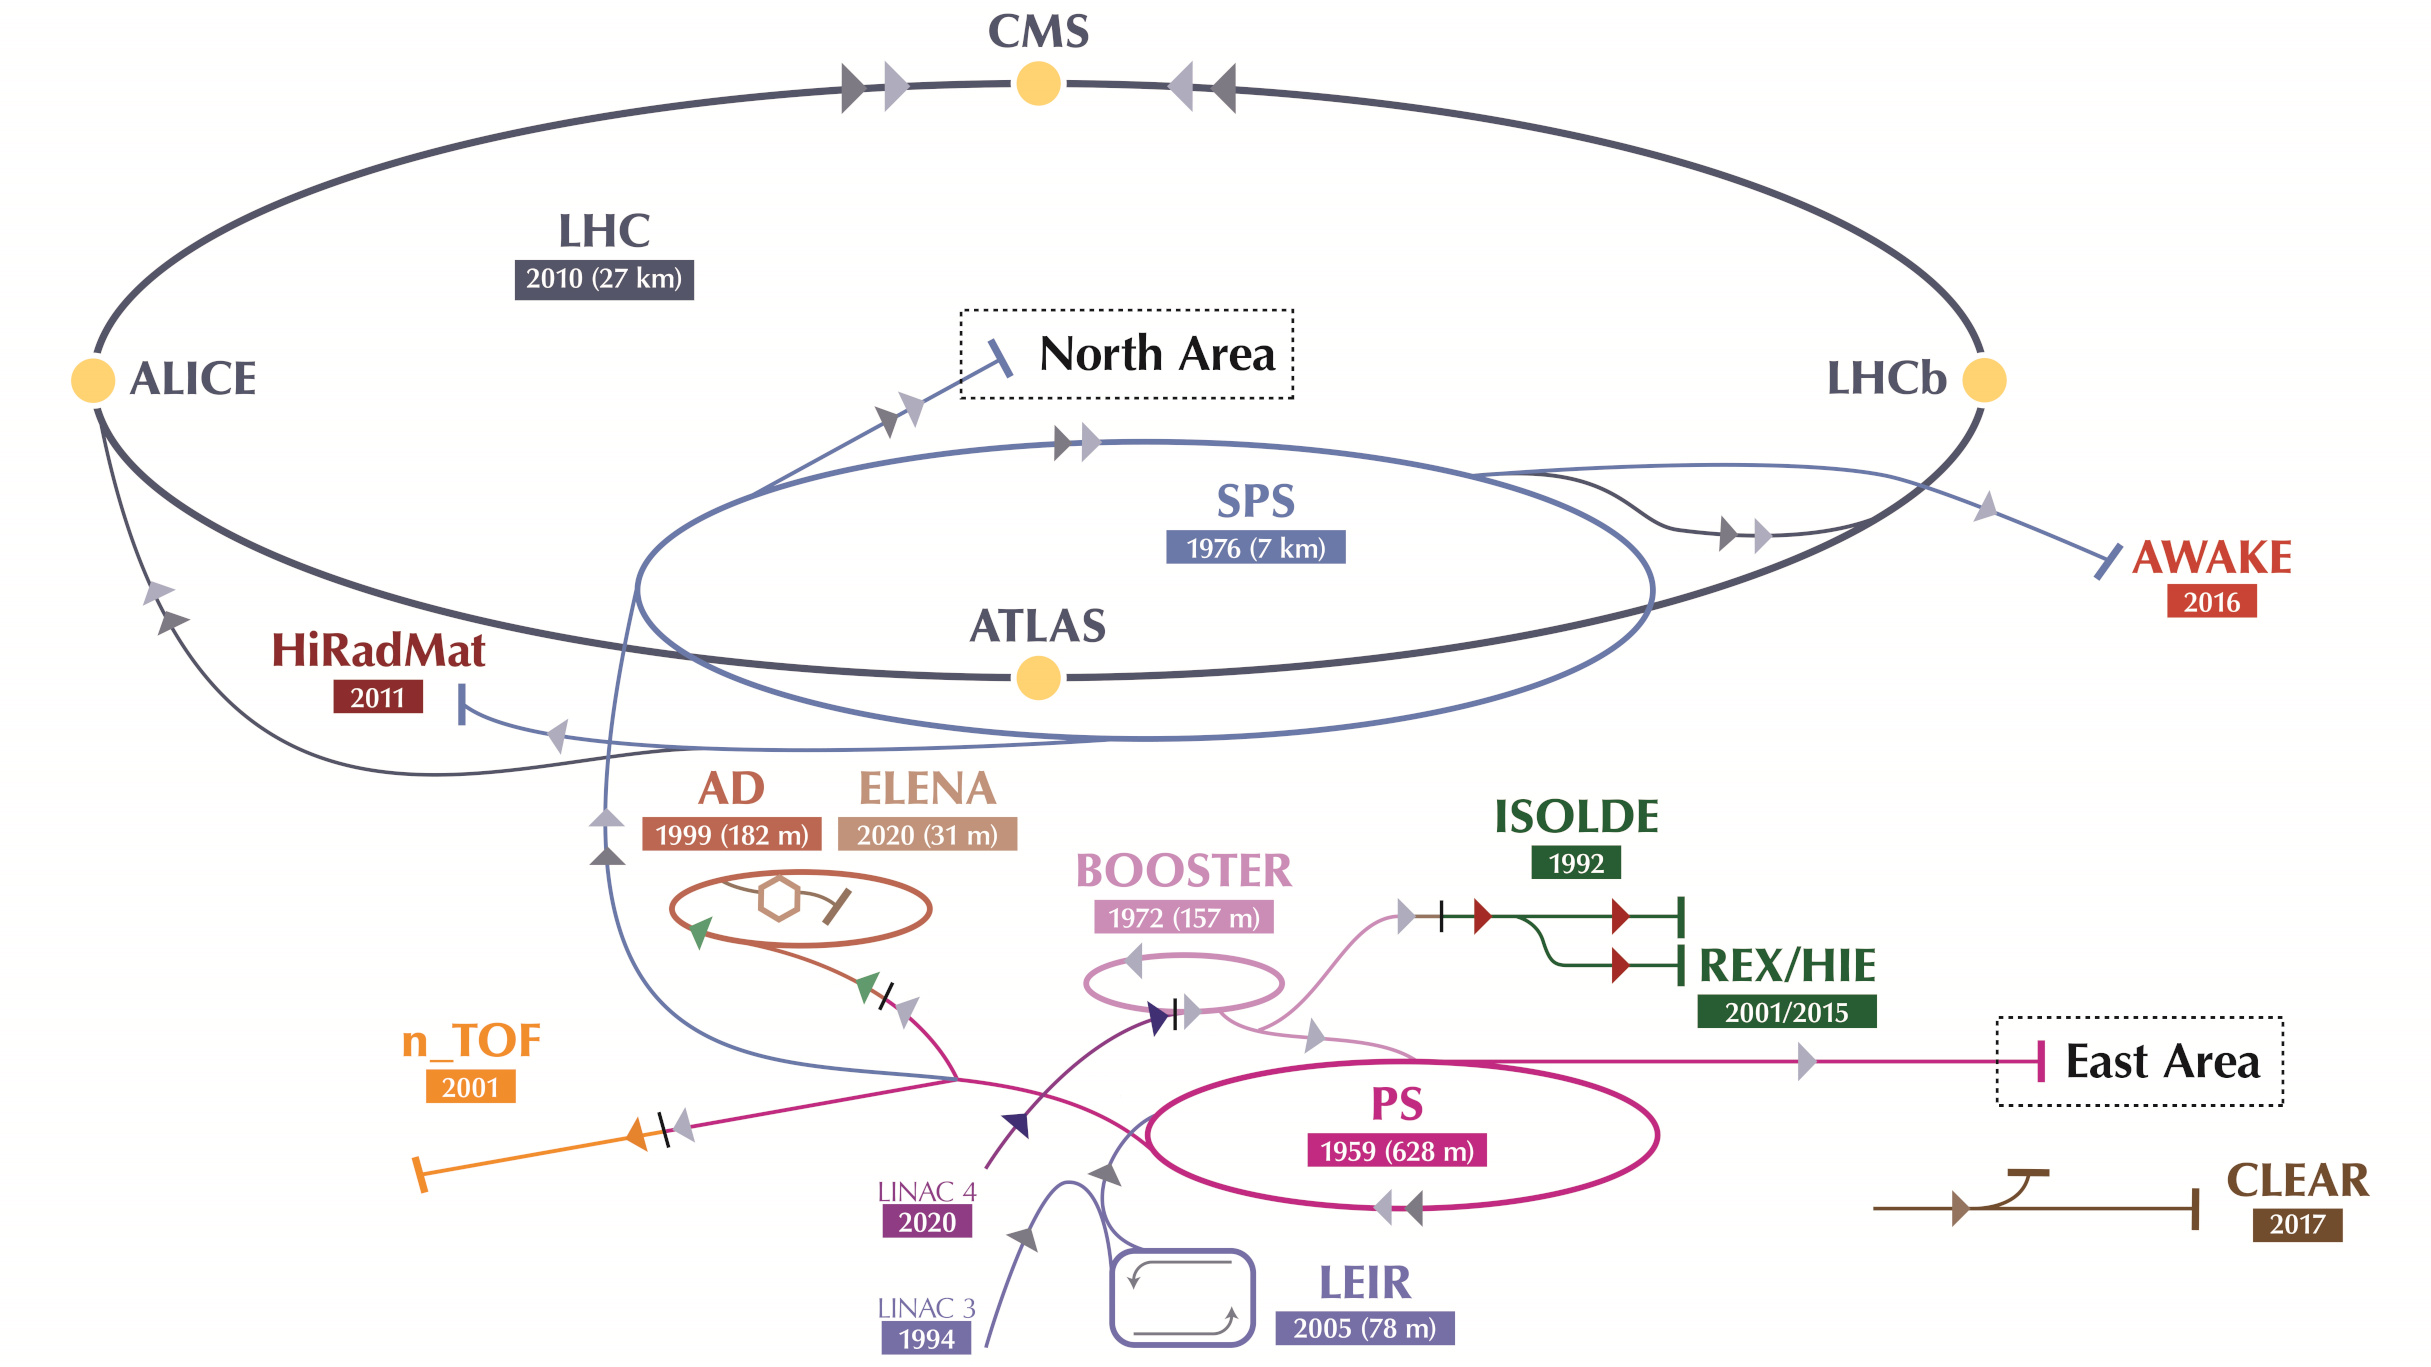
\includegraphics[width=\textwidth]{\PhDthesisdir/plots_and_images/CERN_and_LHC/CERN_Accelerator-Complex_2020.tex}
\caption[Complexe des accélérateurs du CERN.]{Complexe des accélérateurs du CERN~\cite{CERN_website}. 
De nombreuses expériences y sont installées:
AD, Décélérateur d'Antiprotons;
AWAKE, \emph{Advanced WAKefield Experiment};
BOOSTER, Booster du Synchrotron à Protons;
CLEAR, \emph{CERN Linear Electron Accelerator for Research};
ELENA, \emph{Extra Low Energy Antiproton};
HiRadMat, \emph{High-Radiation to Materials};
ISOLDE, \emph{Isotope mass Separator On-Line};
LEIR, Anneau d’Ions de Basse Énergie;
LHC, Grand Collisionneur de Hadrons;
LINAC~3, Accélérateur Linéaire~3;
LINAC~4, Accélérateur Linéaire~4, remplace le LINAC~2;
n\_TOF, \emph{Neutrons Time Of Flight};
PS, Synchrotron à Protons;
REX/HIE, \emph{Radioactive EXperiment/High Intensity and Energy};
SPS, Supersynchrotron à Protons;
ALICE, \emph{A Large Ion Collider Experiment};
ATLAS, \emph{A Toroidal LHC ApparatuS};
CMS, \emph{Compact Muon Solenoid};
LHCb, \emph{Large Hadron Collider beauty}.}
\label{fig-chapter-LHC-section-CERN-CERN_Accelerator-Complex}
\end{figure}